\section{Speciell relativitet}

\paragraph{Galileitransformationen}
Betrakta en statisk ram $S$ och en ram $S'$ som rör sig med konstant hastighet $\vb{u}$. Galileitransformen är den klassiska transformen av hastigheter och accelerationer mellan dessa system och ger
\begin{align*}
	\vb{r} = \vb{u}t + \vb{r}', \\
	\vb{v} = \vb{u} + \vb{v}', \\
	\vb{a} = \vb{a}'. \\
\end{align*}

\paragraph{Michelson-Morleys experiment}
Michelson-Morleys experiment visade att ljus omöjligt kunde propageras genom den postulerade etern.

Uppställningen som användes är (en mer avancerad variant av) Michelson-Morley-interferometern, som illustreras i figur \ref{fig:interferometer}.
\begin{figure}[!ht]
	\centering
	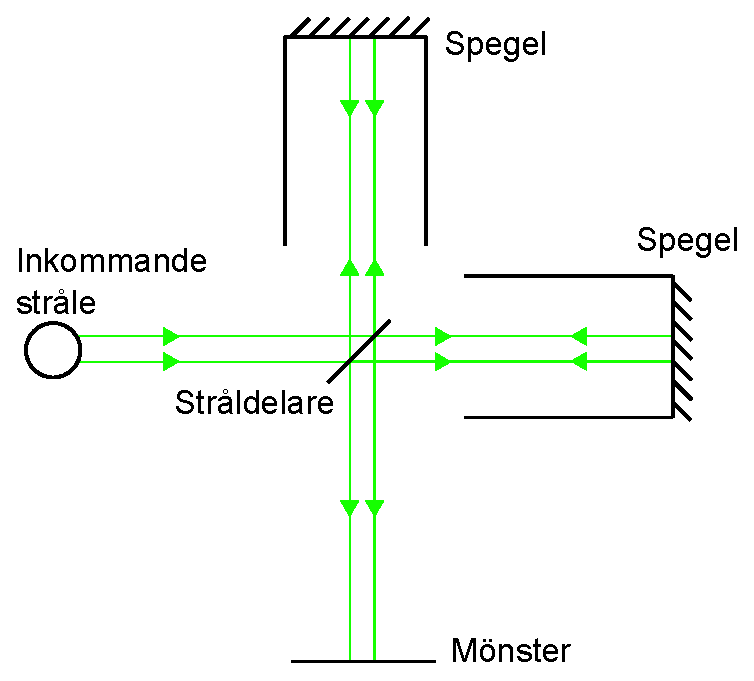
\includegraphics[width = 0.5\textwidth]{./Images/interferometer.eps}
	\caption{}
	\label{fig:interferometer}
\end{figure}

Ideen bakom experimentet var att de två "armarna" i uppställningen skulle röra sig med olika hastigheter relativt etern eftersom Jorden rör sig relativt Solen.

Om nu varje arm har längd $L$ och etern rör sig med en hastighet $u$ åt höger, tar ljuset tiden
\begin{align*}
	t_{\text{höger}} &= \frac{L}{c + u} + \frac{L}{c - u} \\
	                 &= L\frac{c - u + c + u}{c^{2} - u^{2}} \\
	                 &= \frac{2cL}{c^{2} - u^{2}} \\
	                 &= \frac{2L}{c}\frac{1}{1 - \frac{u^{2}}{c^{2}}}
\end{align*}
att röra sig till och från stråldelaren åt höger och tiden
\begin{align*}
	t_{\text{upp}} &= \frac{2L}{\sqrt{c^{2} - u^{2}}} \\
	               &= \frac{2L}{c}\frac{\sqrt{1 - \frac{u^{2}}{c^{2}}}}{1 - \frac{u^{2}}{c^{2}}},
\end{align*}
ty ljuset måste röra sig uppåt och motriktad hastigheten mot höger för att återvända till samma position i stråldelaren. Alltså borde skillnaden mellan tiden det tar för ljuset att röra sig de två vägarna ges av
\begin{align*}
	\Delta t = \frac{2L}{c}\frac{1 - \sqrt{1 - \frac{u^{2}}{c^{2}}}}{1 - \frac{u^{2}}{c^{2}}}.
\end{align*}
För Michelson och Morleys fal förutspådde de att de skulle se $0.4$ fransar i interferensmönstret, men de observerade $< 0.01$ fransar. Efter att ha upprepat sitt experiment ett halvår senare för att utesluta påverkan från Jordens position, konkluderade de med att det inte kunde finnas någon eter.

\paragraph{Einsteins postulat}
Baserad på Michelson-Morleys experiment, kom Einstein med följande postulat:
\begin{itemize}
	\item Fysikens lagar är de samma i alla inertialsystem.
	\item Ljushastigheten i vakuum har samma värde $c$ i alla inertialsystem.
\end{itemize}

\paragraph{Lorentztransformationen}
Lorentztransformationen är en transformation för att byta mellan olika referensramer. Den skiljer sig från Galileitransformationer, som inte är tillräcklig för att beskriva denna nya fysiken.

För att härleda Lorentztransformationen, betrakta två referensramar som sammanfallar vid $t = 0$ där den ena rör sig med en hastighet $v$ i $x$-riktning. För att beskriva transformationen, ansätter vi
\begin{align*}
	x' = k_{i}x_{i},
\end{align*}
där det summeras över alla rymdliga koordinater och tiden. Vi ansätter linjaritet eftersom det annars skulle kunna uppkomma accelererande rörelse i ett system utan att det är acceleration i ett annat, vilket skulle vara konstigt. Vidare antar vi att $x'$ ej beror av andra rymdliga kordinater, men att den kan bero av origos rörelse, och ansätter
\begin{align*}
	x' = k_{1}(x - vt).
\end{align*}
Antag nu att vi skickar ut en ljuspuls från origo vid $t = 0$. Vågfrontens avstånd från origo kommer beskrivas av
\begin{align*}
	x^{2} + y^{2} + z^{2} = c^{2}t^{2},
	x'^{2} + y^{2} + z^{2} = c^{2}t'^{2},
\end{align*}
eftersom ljuset skall ha samma fart i båda referensramer. Vi använder nu våran ansats för att transformera den andra ekvationen tillbaka, och får
\begin{align*}
	k_{1}^{2}x^{2} + y^{2} + z^{2} + k_{1}^{2}(v^{2}t^{2} - 2xvt) = c^{2}t'^{2}.
\end{align*}
Om vi sätter $t = t'$, får vi nu andra termer, och transformationen mislyckades. Vi åtgärder detta vid att ansätta
\begin{align*}
	t' = k_{t, 1}x + k_{t, 2}t.
\end{align*}
Detta ger
\begin{align*}
	k_{1}^{2}x^{2} + y^{2} + z^{2} + k_{1}^{2}(v^{2}t^{2} - 2xvt) = c^{2}(k_{t, 1}^{2}x^{2} + k_{t, 2}^{2}t^{2} + 2k_{t, 1}k_{t, 2}xt).
\end{align*}
För att transformationen skall lyckas, ger detta
\begin{align*}
	k_{1}^{2} - c^{2}k_{t, 1}^{2} = 1, \\
	vk_{1}^{2} + k_{t, 1}k_{t, 2}c^{2} = 0, \\
	c^{2}k_{t, 2}^{2} - k_{1}^{2}v^{2} = 0.
\end{align*}
Vid att införa
\begin{align*}
	\beta = \frac{v}{c}, \gamma = \frac{1}{\sqrt{1 - \beta^{2}}}
\end{align*}
kan lösningarna skrivas som
\begin{align*}
	k_{1} = k_{t, 2} = \gamma, k_{t, 1} = -\frac{\beta\gamma}{c}.
\end{align*}
Lorentztransformationerna ges då av
\begin{align*}
	x' = \gamma(x - vt), t' = \gamma\left(t - \frac{\beta}{c}x\right).
\end{align*}
Den inversa Lorentztransformationen fås vid att lösa ut ekvationerna för $x$ och $t$, och ges av
\begin{align*}
	x = \gamma(x' + vt'), t = \gamma(t' + \frac{\beta}{c}x').
\end{align*}
Med de givna skalfaktorerna ser vi att för små hastigheter går detta över i Galileitransformer, medan inga hastigheter över $c$ tillåts.

\paragraph{Samtidighet}
Betrakta två händelser som inträffer vid olika tidspunkter och positioner. Lorentztransformationen ger
\begin{align*}
	\Delta t = \gamma(\Delta t' + \frac{\beta}{c}\Delta x').
\end{align*}
Detta implicerar att om händelserna är samtidiga i en referensram, är de inte nödvändigtvis det i den andra.

\paragraph{Tidsdilation}
Betrakta två händelser som inträffer vid samma position i den rörliga ramen. Lorentztransformationen ger
\begin{align*}
	\Delta t = \gamma\Delta t',
\end{align*}
och det mäts en längre tidsskilland mellan händelserna i inertialramen.

\paragraph{Längdkontraktion}
Betrakta två händelser som inträffer vid samma tidspunkt i inertialramen. Lorentztransformationen ger
\begin{align*}
	\Delta x = \frac{1}{\gamma}\Delta x,
\end{align*}
och det mäts ett kortare avstånd mellan händelserna i inertialramen.

\paragraph{Relativistisk Dopplereffekt}
Betrakta återigen två olika system. Från $O'$ skickas det ut ljuspulser vid $t_{1}'$ och $t_{2}'$. Lorentztransformationerna ger att ljuset skickas ut vid tider
\begin{align*}
	t_{1} = \gamma t_{1}', \\
	t_{2} = \gamma t_{2}'
\end{align*}
och vid avstånd
\begin{align*}
	x_{1} = \gamma vt_{1}', \\
	x_{2} = \gamma vt_{2}'.
\end{align*}
Ljuspulserna når därmed origo vid tid
\begin{align*}
	t_{O1} = t_{1} + \frac{x_{1}}{c} = \gamma t_{1}'(1 + \beta), \\
	t_{O2} = t_{2} + \frac{x_{2}}{c} = \gamma t_{2}'(1 + \beta).
\end{align*}
Vi inför periodtiden $\Delta t' = t_{2}' - t_{1}'$, och får
\begin{align*}
	\Delta t_{O} = \gamma (1 + \beta)\Delta t'.
\end{align*}
Frekvensen för ljuspulsen ges då av
\begin{align*}
	f_{\text{obs}} = \frac{1}{\gamma(1 + \beta)}f_{\text{källa}}.
\end{align*}

\paragraph{Lorentztransformation av hastigheter}
Vi använder differentialerna
\begin{align*}
	\dd{x} = \gamma(\dd{x'} + v\dd{t'}), \\
	\dd{t} = \gamma(\dd{t'} + \frac{\beta}{c}\dd{x'})
\end{align*}
och får hastigheterna
\begin{align*}
	u_{x} &= \dv{x}{t} = \frac{\dd{x'} + v\dd{t'}}{\dd{t'} + \frac{\beta}{c}\dd{x'}} = \frac{u_{x}' + v}{1 + \frac{\beta}{c}u_{x}'}, \\
	u_{y} &= \frac{u_{y}'}{1 + \frac{\beta}{c}u_{x}'}, \\
	u_{z} &= \frac{u_{z}'}{1 + \frac{\beta}{c}u_{x}'}.
\end{align*}

\paragraph{Relativistisk rörelsemängd}
Betrakta studsen som illustreras i figur \ref{fig:collision_inertial}.
\begin{figure}[!ht]
	\centering
	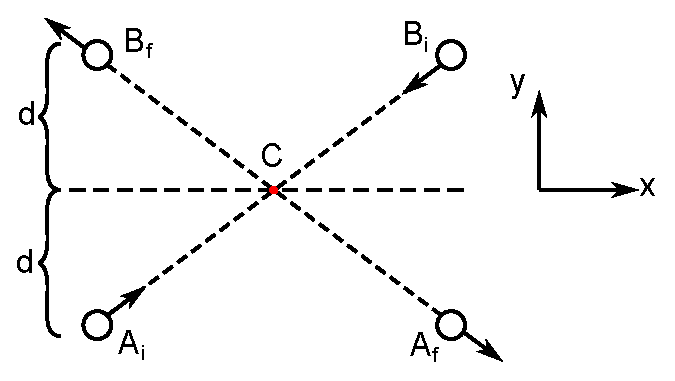
\includegraphics[width = 0.5\textwidth]{./Images/collision_inertial.eps}
	\caption{Illustration}
	\label{fig:collision_inertial}
\end{figure}

Vi antar här att rörelsen kan vara relativistisk i $x$, men approximeras som klassisk i $y$. Om partiklerna har samma massa (och hastighet), är masscentrum statiskt i $C$.

Vi kan alternativt betrakta studsen i ett system som följer partikeln $A$ i $x$-riktning, vilket illustreras i figur \ref{fig:collision_following}.
\begin{figure}[!ht]
	\centering
	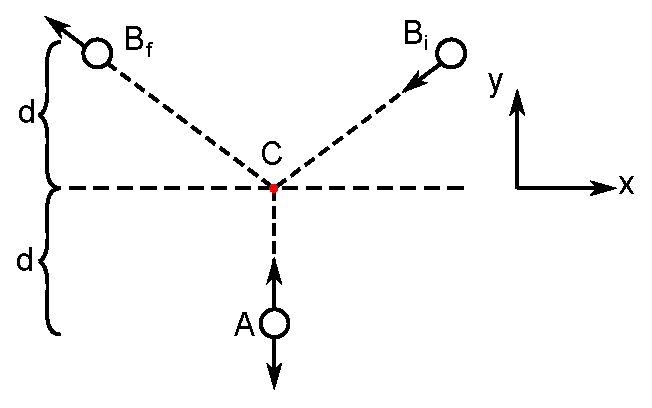
\includegraphics[width = 0.5\textwidth]{./Images/collision_following.eps}
	\caption{Illustration}
	\label{fig:collision_following}
\end{figure}

Båda system är inertialsystem, och därmed är rörelsesmängden bevarad i båda system.

Vi definierar tiden $t_{0}$ som det tar för $A$ att röra sig avståndet $d$ upp och ned i $A$:s referensram. Ändringen i rörelsemängd ges då av
\begin{align*}
	\Delta p_{A, y} = -2m_{A}\frac{d}{t_{0}} - 2m_{A}\frac{d}{t_{0}} = -4m_{A}\frac{d}{t_{0}}, \\
	\Delta p_{B, y} = 2m_{B}\frac{d}{t_{0}} + 2m_{B}\frac{d}{t_{0}} = 4m_{B}\frac{d}{t},
\end{align*}
där tiden $t$ är tiden det tar för $B$ att röra sig upp och ned i den betraktade referensramen. Eftersom rörelsen i $y$-riktning är klassisk, är denna tiden $t_{0}$ i $B$:s referensram. Vi transformerar därmed tillbaka och får
\begin{align*}
	\Delta p_{B, y} = 4m_{B}\frac{d}{\gamma t_{0}}.
\end{align*}
Fysikens lagar gäller i alla inertialsystem, vilket systemet vi betraktar är, och därmed är den totala ändringen i rörelsemängdsmoment lika med $0$, vilket ger
\begin{align*}
	m_{B} = \gamma m_{A}.
\end{align*}
Eftersom rörelsen i $y$-riktning är klassisk, kan $A$:s massa nu ersättas av vilomassan $m_{0}$, som är $A$:s massa mätt i sitt eget inertialsystem. Eftersom de två har samma vilomassa, ger detta
\begin{align*}
	m = \gamma m_{0}.
\end{align*}
Den relativistiska rörelsemängden ges därmed av
\begin{align*}
	p = mv = \gamma m_{o}v.
\end{align*}

\paragraph{Relativistisk energi}
Newtons andra lag ger
\begin{align*}
	F = \dv{t}\left(mv\right).
\end{align*}
Om kraftsumman $F$ får verka på en partikel som börjar från vilo, ges dens kinetiska energi av
\begin{align*}
	T = \int F\cdot\dd{s} = \int\dv{t}\left(mv\right)\cdot v\dd{t} = \int v\cdot\dd{(mv)} = \int v^{2}\dd{m} + mv\cdot\dd{v}.
\end{align*}
Lorentztransformationen av massa ger
\begin{align*}
	m^{2}\gamma^{2} = m_{0}^{2}, m^{2}(c^{2} - v^{2}) = m_{0}^{2}c^{2}.
\end{align*}
Vid att beröäkna differentialen av båda sidor får
\begin{align*}
	2mc^{2}\dd{m} - 2mv^{2}\dd{m} - 2m^{2}v\cdot\dd{v} = 0, c^{2}m = v^{2}\dd{m} + mv\cdot\dd{v},
\end{align*}
vilket insatt i integralen ger
\begin{align*}
	T = \int c^{2}\dd{m} = c^{2}(m - m_{0}) = m_{0}c^{2}(\gamma - 1).
\end{align*}
Detta kan alternativt skrivas som
\begin{align*}
	mc^{2} = T + m_{0}c^{2},
\end{align*}
vilket tolkades som ett uttryck för totala energin som innehåller en konstant viloenergi $m_{0}c^{2}$ (obs: Ej en potentiell energi!). Därmed ges den totala energin av
\begin{align*}
	E = mc^{2} = T + m_{0}c^{2}.
\end{align*}

\paragraph{Relation mellan energi och rörelsemängd}
Vi har nu fått
\begin{align*}
	p^{2} = \gamma^{2}m_{0}^{2}v^{2}, E^{2} = \gamma^{2}m_{0}^{2}c^{4}.
\end{align*}
Energin i kvadrat kan skrivas som
\begin{align*}
	E^{2} = \gamma^{2}m_{0}^{2}c^{4} = \gamma^{2}m_{0}^{2}c^{4}\left(\frac{1}{\gamma^{2}} + \beta^{2}\right),
\end{align*}
eftersom $\gamma = \frac{1}{\sqrt{1 - \beta^{2}}}$. Vi får vidare
\begin{align*}
	E^{2} &= m_{0}^{2}c^{4} + m_{0}^{2}v^{2}c^{2} \\
	      &= m_{0}^{2}c^{4} + p^{2}c^{2}.
\end{align*}